\documentclass[a4paper,oneside,12pt]{report}
% Package yang diperlukan
\usepackage{fontspec}       % Font sistem untuk XeLaTeX/LuaLaTeX
\usepackage{setspace}       % Pengaturan jarak antarbaris
\usepackage{graphicx}      % Untuk memasukkan gambar
\usepackage{titling}       % Untuk kustomisasi halaman judul
\usepackage{geometry}      % Untuk mengatur margin halaman
\usepackage{listings}      % Untuk menampilkan blok kode
\usepackage{xcolor}        % Untuk menggunakan warna
\usepackage{float}         % Untuk kontrol penempatan float (seperti gambar)
\usepackage{hyperref}      % Untuk membuat hyperlink (URL, referensi)
\usepackage{indentfirst}   % Untuk memberi indentasi pada paragraf pertama setiap seksi
\usepackage{url}           % Untuk format URL
\usepackage{fancyhdr}      % Untuk kustomisasi header dan footer
\usepackage{tocloft}       % Untuk kustomisasi Daftar Isi
\usepackage{bookmark}      % Untuk manajemen bookmark PDF yang lebih baik

% Font dan spasi standar laporan praktikum
\setmainfont{Times New Roman}
\onehalfspacing

%======================================================================
% PENGATURAN GEOMETRI HALAMAN
%======================================================================
% Margin umum untuk isi laporan
\geometry{left=3cm, right=2.5cm, top=2cm, bottom=2.5cm}
\sloppy

%======================================================================
% PENGATURAN WARNA UNTUK BLOK KODE
%======================================================================
\definecolor{codegreen}{rgb}{0,0.6,0}
\definecolor{codegray}{rgb}{0.5,0.5,0.5}
\definecolor{codepurple}{rgb}{0.58,0,0.82}
\definecolor{backcolour}{rgb}{0.95,0.95,0.92}
\definecolor{darkblue}{rgb}{0,0,0.6}

%======================================================================
% PENGATURAN BLOK KODE (LISTINGS)
%======================================================================
% Gaya umum untuk semua blok kode
\lstdefinestyle{commonstyle}{
    backgroundcolor=\color{backcolour}, 
    breakatwhitespace=false, 
    breaklines=true, 
    captionpos=b, 
    keepspaces=true,
    numbers=left, 
    numbersep=5pt, 
    showspaces=false, 
    showstringspaces=false,
    showtabs=false, 
    tabsize=2, 
    frame=single,
    basicstyle=\ttfamily\footnotesize,
    numberstyle=\tiny\color{codegray},
    columns=flexible,
    postbreak=\mbox{\textcolor{red}{$\hookrightarrow$}\space},
    breakindent=0pt,
    breakautoindent=false
}

% Gaya khusus untuk HTML
\lstdefinestyle{htmlstyle}{
    style=commonstyle,
    language=HTML,
    commentstyle=\color{codegreen},
    keywordstyle=\color{codepurple},
    stringstyle=\color{codegreen},
    basicstyle=\ttfamily\scriptsize
}

% Gaya khusus untuk CSS
\lstdefinestyle{cssstyle}{
    style=commonstyle,
    commentstyle=\color{codegreen},
    keywordstyle=\color{darkblue},
    stringstyle=\color{codepurple},
    emph={color, background, font, margin, padding, border, display, position, width, height},
    emphstyle=\color{darkblue},
    basicstyle=\ttfamily\scriptsize
}

% Gaya khusus untuk Python
\lstdefinestyle{pythonstyle}{
    style=commonstyle,
    language=Python,
    commentstyle=\color{codegreen},
    keywordstyle=\color{darkblue},
    stringstyle=\color{codepurple},
    emph={import,from,class,def,for,while,if,else,elif,try,except,finally},
    emphstyle=\color{darkblue}
}

% Gaya khusus untuk SQL
\lstdefinestyle{sqlstyle}{
    style=commonstyle,
    language=SQL,
    commentstyle=\color{codegreen},
    keywordstyle=\color{darkblue},
    stringstyle=\color{codepurple},
    emph={SELECT,FROM,WHERE,INSERT,UPDATE,DELETE,CREATE,DROP},
    emphstyle=\color{darkblue}
}

% Gaya khusus untuk JavaScript
\lstdefinestyle{javascriptstyle}{
    style=commonstyle,
    language=JavaScript,
    commentstyle=\color{codegreen},
    keywordstyle=\color{darkblue},
    stringstyle=\color{codepurple},
    emph={function,var,let,const,return,if,for,while,do,else,switch,case},
    emphstyle=\color{darkblue}
}

%======================================================================
% PENGATURAN LAIN-LAIN
%======================================================================
% Perintah kustom untuk bingkai gambar
\newcommand{\customfbox}[1]{%
  \setlength{\fboxsep}{0pt}%
  \setlength{\fboxrule}{0.5pt}%
  \fcolorbox{black}{white}{#1}%
}

% Mengganti nama default "Figure" menjadi "Gambar"
\renewcommand{\figurename}{Gambar}
\renewcommand{\thefigure}{\arabic{figure}}

% Pengaturan Hyperlink
\hypersetup{
    colorlinks=true, 
    linkcolor=black, 
    filecolor=black, 
    urlcolor=black,
    citecolor=black,
    pdftitle={Laporan Praktikum}, 
    pdfpagemode=FullScreen, 
    breaklinks=true
}

% Pengaturan Header & Footer (nomor halaman di tengah bawah)
\pagestyle{fancy}
\fancyhf{}
\fancyfoot[C]{\thepage}
\renewcommand{\headrulewidth}{0pt}

\fancypagestyle{plain}{
    \fancyhf{}
    \fancyfoot[C]{\thepage}
    \renewcommand{\headrulewidth}{0pt}
}

%======================================================================
% PENGATURAN STRUKTUR BAB DAN DAFTAR ISI
%======================================================================
\renewcommand{\contentsname}{Daftar Isi}
\renewcommand{\bibname}{Daftar Pustaka}

% Menghilangkan nomor bab tetapi mempertahankan penomoran seksi
\renewcommand{\thechapter}{}
\renewcommand{\chaptername}{}

% Format penomoran seksi menjadi [nomor bab].[nomor seksi]
\renewcommand{\thesection}{\arabic{chapter}.\arabic{section}}
\renewcommand{\thesubsection}{\thesection.\arabic{subsection}}

\setcounter{secnumdepth}{3}
\setcounter{tocdepth}{3}

% Format Daftar Isi (TOC)
\renewcommand{\cftchapdotsep}{\cftdotsep}
\renewcommand{\cftchapleader}{\cftdotfill{\cftchapdotsep}}
\setlength{\cftchapindent}{0em}
\setlength{\cftsecindent}{2em}
\setlength{\cftsubsecindent}{4em}
\setlength{\cftchapnumwidth}{0em}
\setlength{\cftsecnumwidth}{2.5em}
\setlength{\cftsubsecnumwidth}{3.2em}
\renewcommand{\cftchappresnum}{}
\renewcommand{\cftchapaftersnum}{}

% Perintah kustom untuk membuat judul bab di TOC menjadi tebal
\newcommand{\tocboldsection}[1]{%
  \protect\renewcommand{\protect\cftchapfont}{\protect\bfseries}%
  #1%
  \protect\renewcommand{\protect\cftchapfont}{}%
}

%======================================================================
% AWAL DOKUMEN
%======================================================================
\begin{document}

% Halaman Judul
\newgeometry{left=3cm, right=2.5cm, top=2.5cm, bottom=3cm}
\begin{titlingpage}
\begin{spacing}{1}
\begin{center}
\vspace*{0.2cm}
{\large \textbf{\MakeUppercase{Laporan Praktikum}}} \\[0.4cm]
{\large \textbf{\MakeUppercase{PRAKTIKUM
PENAMBANGAN DATA}}} \\[0.4cm]
{\large \textbf{\MakeUppercase{Pertemuan 1}}} \\[0.4cm]
{\large \textbf{\MakeUppercase{PENGENALAN NUMPY DAN PANDAS}}} \\[1.5cm]


\includegraphics[height=7cm]{../template-pertemuan/images/UGM.png} \\[0.7cm]

{\normalsize \textbf{Disusun oleh:}} \\[0.4cm]
\begin{tabular}{@{}l l @{}}
  \textbf{Nama}           & : Hafidz Rizqullah Prasetya \\
  \textbf{NIM}            & : 24/535493/SV/24243 \\
  \textbf{Kelas}          & : PL5A1 \\
  \textbf{Dosen Pengampu} & : Dr. Imam Fahrurrozi, S.T., M.Cs.
\end{tabular} \\[1.2cm]

{\normalsize \textbf{PROGRAM STUDI D-IV}} \\[0.2cm]
{\normalsize \textbf{TEKNOLOGI REKAYASA PERANGKAT LUNAK}} \\[0.2cm]
{\normalsize \textbf{DEPARTEMEN TEKNIK ELEKTRO DAN INFORMATIKA}} \\[0.2cm]
{\normalsize \textbf{SEKOLAH VOKASI}} \\[0.2cm]
{\normalsize \textbf{UNIVERSITAS GADJAH MADA}} \\[0.2cm]
{\normalsize \textbf{YOGYAKARTA}} \\[0.2cm]
{\normalsize \textbf{2026}} \\[1.2cm]
\end{center}
\end{spacing}
\end{titlingpage}
\restoregeometry

\thispagestyle{empty}
\clearpage
\stepcounter{page}
\thispagestyle{empty}

% --- Daftar Isi ---
\addcontentsline{toc}{chapter}{Daftar Isi}
\tableofcontents
\clearpage

% Mengatur penomoran halaman menjadi arab dan mulai dari 3
\pagenumbering{arabic}
\setcounter{page}{3}

\chapter[Tujuan Praktikum]{Tujuan Praktikum}
\begin{enumerate}
   \item Mahasiswa mampu menjelaskan konsep dasar NumPy, membuat array berdimensi-N, serta melakukan indexing, slicing, reshape, penggabungan, pencarian, pengurutan, dan operasi numerik pada array.
   \item Mahasiswa mampu menjelaskan struktur data Series dan DataFrame serta melakukan manipulasi dan transformasi data menggunakan pandas.
   \item Mahasiswa mampu menerapkan NumPy dan pandas untuk mengolah, meringkas, dan menganalisis data tabular.
\end{enumerate}
\clearpage

\chapter{Dasar Teori}

\section{NumPy}

\subsection{Pengertian NumPy dan Array ndarray}
NumPy merupakan pustaka Python sumber terbuka yang digunakan untuk komputasi
numerik. Struktur data utama NumPy adalah \textit{ndarray}, yaitu array
berdimensi-N yang menyimpan elemen dengan tipe data yang homogen. Berbeda
dengan list Python yang dapat menyimpan elemen dengan tipe berbeda, array NumPy
dirancang untuk menyimpan data sejenis secara efisien. Karakteristik tersebut
mendukung operasi numerik pada data dalam jumlah besar \cite{numpy-basics,petanikode-numpy}.

Istilah \textit{ndarray} merupakan singkatan dari \textit{N-dimensional array}.
Istilah ini bukan pustaka yang terpisah, melainkan tipe objek array yang
digunakan NumPy untuk merepresentasikan data satu dimensi, dua dimensi, atau
lebih. Oleh karena itu, pembahasan array NumPy pada praktikum ini merujuk pada
objek \textit{ndarray}.

\begin{figure}[H]
    \centering
    \fbox{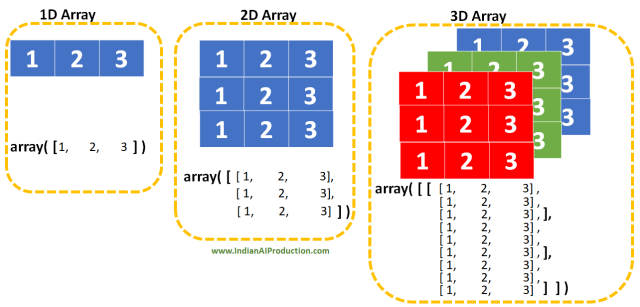
\includegraphics[width=0.8\textwidth]{images/image.png}}
    \caption{Ilustrasi array NumPy 1D, 2D, dan 3D.}
    \label{fig:ndarray-dimensi}
\end{figure}

Array NumPy dapat dibuat dari sekuens Python, seperti list dan \textit{nested
list}, menggunakan fungsi \texttt{np.array()}. Array satu dimensi dapat
digunakan untuk merepresentasikan deret data, sedangkan array dua dimensi dapat
digunakan untuk merepresentasikan tabel. Penambahan tingkat kemanunggalan
struktur menghasilkan array tiga dimensi atau lebih.

\subsection{Dimensi, shape, size, dan dtype}
Array mempunyai beberapa atribut penting. Atribut \texttt{ndim} menyatakan
jumlah dimensi atau sumbu array. Atribut \texttt{shape} menghasilkan tuple yang
menyatakan jumlah elemen pada setiap sumbu. Atribut \texttt{size} menyatakan
jumlah seluruh elemen, sedangkan \texttt{dtype} menyatakan tipe data elemen
array. Sebagai contoh, array dengan \texttt{shape} \texttt{(2, 3)} mempunyai
dua baris dan tiga kolom, sehingga jumlah elemennya adalah enam
\cite{numpy-basics}.

Pemahaman terhadap \texttt{shape} penting ketika array akan diubah bentuknya
atau digabungkan. Operasi \texttt{reshape()} hanya dapat dilakukan apabila
jumlah elemen sebelum dan sesudah perubahan tetap sama. Dengan demikian, array
yang mempunyai dua belas elemen dapat diubah menjadi bentuk \texttt{(3, 4)}
atau \texttt{(2, 6)}, tetapi tidak menjadi bentuk yang jumlah elemennya bukan
dua belas.

\subsection{Indexing dan slicing}
Indexing digunakan untuk mengambil satu elemen berdasarkan posisinya. NumPy
menggunakan indeks berbasis nol, sehingga elemen pertama berada pada indeks
\texttt{0}. Pada array dua dimensi, elemen dapat diakses dengan format
\texttt{array[baris, kolom]}. Pada array dengan lebih banyak dimensi, indeks
diberikan untuk setiap sumbu secara berurutan.

Slicing digunakan untuk mengambil sebagian array menggunakan format batas awal,
batas akhir, dan langkah, misalnya \texttt{array[1:4]}. Batas akhir tidak
termasuk dalam hasil slicing. Slicing juga dapat diterapkan pada beberapa
sumbu, misalnya \texttt{array[2, 1:, 0]}. Pada banyak kasus, hasil slicing
NumPy berupa \textit{view} terhadap data asal, bukan salinan baru. Oleh karena
itu, perubahan pada hasil slicing dapat memengaruhi array asal
\cite{numpy-basics}.

\begin{figure}[H]
    \centering
    \fbox{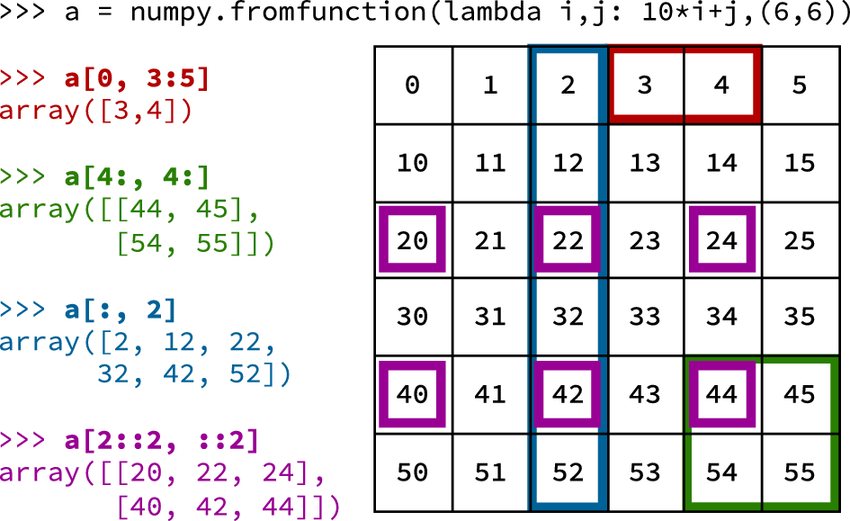
\includegraphics[width=0.8\textwidth]{images/image copy.png}}
    \caption{Contoh indexing dan slicing pada array NumPy.}
    \label{fig:ndarray-indexing}
\end{figure}

\subsection{Operasi dan manipulasi array}
NumPy menyediakan operasi element-wise, yaitu operasi yang diterapkan pada
elemen-elemen yang bersesuaian, seperti penjumlahan, pengurangan, perkalian,
dan pembagian. Fungsi \texttt{np.add()} dapat digunakan untuk penjumlahan dua
array. Fungsi agregasi seperti \texttt{np.sum()}, \texttt{np.prod()},
\texttt{np.min()}, \texttt{np.max()}, dan \texttt{np.mean()} digunakan untuk
meringkas nilai array. Parameter \texttt{axis} dapat digunakan untuk
menentukan sumbu tempat operasi dilakukan \cite{numpy-basics}.

Beberapa fungsi manipulasi yang digunakan dalam praktikum adalah
\texttt{np.concatenate()} untuk menggabungkan array, \texttt{np.array\_split()}
untuk membaginya menjadi beberapa bagian, \texttt{np.where()} untuk mencari
posisi elemen yang memenuhi kondisi, dan \texttt{np.sort()} untuk mengurutkan
elemen. NumPy juga menyediakan modul random untuk menghasilkan bilangan
\textit{pseudo-random} dengan bentuk array tertentu. Penggunaan seed dapat
membuat hasil percobaan dapat diulang.

\section{Pandas}

\subsection{Pengertian Series dan DataFrame}
Pandas merupakan pustaka Python untuk pengolahan dan analisis data tabular.
Pandas menyediakan dua struktur data utama, yaitu \textit{Series} dan
\textit{DataFrame}. Series adalah array satu dimensi yang memiliki label,
sedangkan DataFrame adalah struktur data dua dimensi yang memiliki baris dan
kolom. Setiap kolom DataFrame dapat mempunyai tipe data yang berbeda, sehingga
DataFrame sesuai untuk merepresentasikan dataset tabular
\cite{pandas-ten-minutes}.

DataFrame dapat dibuat dari list, dictionary, array NumPy, atau data terstruktur
lainnya. Label baris disebut indeks dan label kolom digunakan untuk mengenali
variabel. Indeks dapat dibuat secara otomatis atau ditentukan secara manual
ketika DataFrame dibuat.

\begin{figure}[H]
    \centering
    \fbox{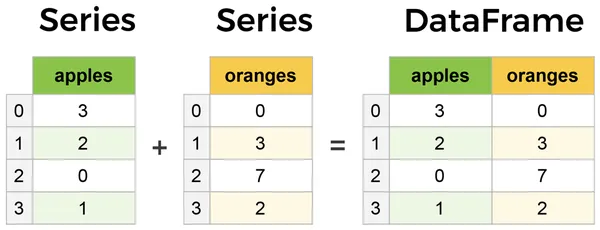
\includegraphics[width=0.8\textwidth]{images/image copy 2.png}}
    \caption{Perbandingan struktur Series dan DataFrame pada pandas.}
    \label{fig:series-dataframe}
\end{figure}

\subsection{Seleksi, penambahan, dan penghapusan data}
Kolom baru dapat ditambahkan menggunakan assignment seperti
\texttt{df['Status'] = nilai}. Fungsi \texttt{insert()} dapat digunakan apabila
kolom perlu ditempatkan pada posisi tertentu. Beberapa kolom dapat ditambahkan
sekaligus menggunakan \texttt{assign()} atau dengan menggabungkan DataFrame
kolom baru menggunakan \texttt{concat()}.

Kolom dapat dihapus menggunakan \texttt{drop()}, \texttt{pop()}, atau
perintah \texttt{del}. Fungsi \texttt{drop()} dapat menghapus satu atau
beberapa kolom. Perbedaan pentingnya adalah \texttt{pop()} menghapus sekaligus
mengembalikan kolom yang dihapus, sedangkan \texttt{drop()} mengembalikan
DataFrame hasil penghapusan apabila tidak digunakan dengan
\texttt{inplace=True}.

DataFrame dapat diurutkan berdasarkan indeks menggunakan
\texttt{sort\_index()} atau berdasarkan isi kolom menggunakan
\texttt{sort\_values()}. Penyaringan data dilakukan dengan mask Boolean,
misalnya \texttt{df[df['Gaji'] > 7000000]}. Beberapa kondisi dapat digabungkan
dengan operator \texttt{\&} dan \texttt{|}; setiap kondisi perlu diberi tanda
kurung. Pandas juga menyediakan \texttt{isin()}, \texttt{query()}, dan
\texttt{str.contains()} untuk kebutuhan penyaringan yang lebih spesifik
\cite{pandas-ten-minutes}.

\subsection{Grouping dan aggregation}
Operasi \textit{groupby} mengikuti pola \textit{split-apply-combine}. Data
dibagi menjadi kelompok berdasarkan satu atau beberapa kolom, fungsi tertentu
diterapkan pada setiap kelompok, kemudian hasilnya digabungkan kembali.
Contohnya, data karyawan dapat dikelompokkan berdasarkan kolom
\texttt{Pekerjaan}.

Setelah pengelompokan, fungsi agregasi seperti \texttt{mean()}, \texttt{sum()},
\texttt{min()}, \texttt{max()}, dan \texttt{std()} dapat digunakan untuk
meringkas data numerik. Fungsi \texttt{agg()} memungkinkan beberapa fungsi
agregasi diterapkan sekaligus, termasuk fungsi yang berbeda untuk kolom yang
berbeda. Hasil agregasi membantu membandingkan karakteristik setiap kelompok
secara ringkas \cite{pandas-groupby}.

\begin{figure}[H]
    \centering
    \fbox{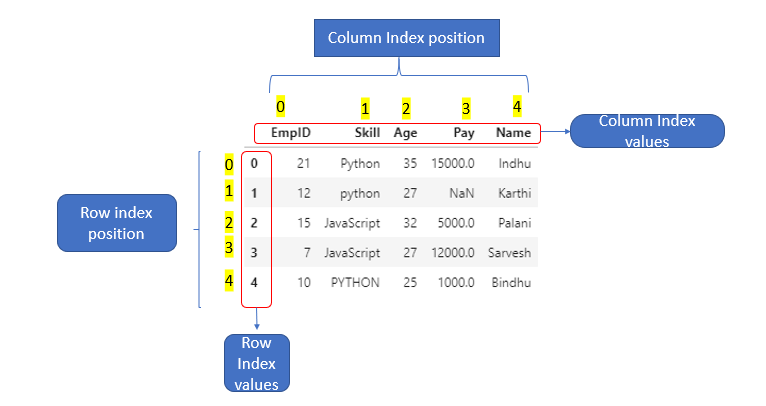
\includegraphics[width=0.8\textwidth]{images/image copy 3.png}}
    \caption{Ilustrasi indeks baris dan kolom pada DataFrame pandas.}
    \label{fig:dataframe-index}
\end{figure}

\subsection{Merge, join, dan concatenate}
Pandas menyediakan beberapa cara untuk menggabungkan DataFrame. Fungsi
\texttt{merge()} melakukan penggabungan berdasarkan kolom kunci atau indeks,
seperti operasi join pada basis data relasional. Parameter \texttt{how} dapat
bernilai \texttt{inner}, \texttt{left}, \texttt{right}, atau \texttt{outer}.
Pada \textit{left join}, seluruh baris dari DataFrame sebelah kiri
dipertahankan, sedangkan data dari DataFrame kanan ditambahkan jika kuncinya
sesuai. Parameter \texttt{left\_on} dan \texttt{right\_on} digunakan ketika
nama kolom kunci pada kedua DataFrame berbeda. Parameter \texttt{suffixes}
digunakan untuk membedakan nama kolom yang sama \cite{pandas-merging}.

Fungsi \texttt{join()} umumnya menggabungkan DataFrame berdasarkan indeks,
sedangkan \texttt{concat()} menyatukan beberapa objek pandas pada sumbu
tertentu. Dengan \texttt{axis=0}, data digabungkan secara vertikal sebagai
baris baru; dengan \texttt{axis=1}, data digabungkan secara horizontal sebagai
kolom baru. Jika label tidak cocok, hasil penggabungan dapat berisi nilai
\texttt{NaN}.

\subsection{Reshaping dan indeks}
Indeks berfungsi sebagai label untuk baris DataFrame. Fungsi
\texttt{reset\_index(drop=True)} mengembalikan indeks menjadi indeks berurutan
dan membuang indeks lama. Sebaliknya, \texttt{set\_index()} menetapkan salah
satu kolom sebagai indeks baru. Pemilihan indeks yang tepat memudahkan akses
data menggunakan \texttt{loc}.

\textit{Pivot table} mengubah susunan data sehingga nilai unik pada kolom
tertentu menjadi indeks atau kolom baru. Fungsi \texttt{pivot\_table()} dapat
melakukan agregasi ketika terdapat lebih dari satu data pada kombinasi indeks
dan kolom. Kebalikan dari format lebar adalah format panjang, yang dapat dibuat
dengan \texttt{melt()}. Pada operasi ini, kolom yang dipertahankan ditentukan
oleh \texttt{id\_vars}, sedangkan kolom yang diubah menjadi pasangan nama dan
nilai ditentukan oleh \texttt{value\_vars} \cite{pandas-reshaping}.

\subsection{Membaca dataset CSV}
CSV adalah format teks untuk menyimpan data tabular dengan pemisah antarnilai.
Pandas menyediakan \texttt{pd.read\_csv()} untuk membaca file CSV menjadi
DataFrame. Setelah selesai diolah, DataFrame dapat disimpan kembali menggunakan
\texttt{to\_csv()}. Dalam Google Colab, file yang berada di Google Drive dapat
diakses setelah Drive di-mount ke lingkungan Colab. Path file kemudian diberikan
sebagai argumen kepada \texttt{pd.read\_csv()} \cite{pandas-io}.

\subsection{Keterkaitan NumPy dan pandas}
NumPy dan pandas saling melengkapi dalam analisis data. NumPy menyediakan array
homogen dan operasi numerik yang efisien, sedangkan pandas menyediakan struktur
berlabel untuk mengelola data tabular. DataFrame pandas dapat dibangun dari
array NumPy dan nilai di dalamnya dapat dikonversi ke representasi NumPy
menggunakan \texttt{to\_numpy()}. Kombinasi keduanya memungkinkan proses mulai
dari pembentukan data, transformasi, peringkasan, hingga analisis dataset.

\clearpage

\chapter[\tocboldsection{Hasil dan Pembahasan}]{Hasil dan Pembahasan}

\section{Percobaan Latihan Praktikum}


\subsection{}


\begin{enumerate}
    \item \textbf{}

    \begin{figure}[H]
        \centering
        \fbox{
\includegraphics[width=1\textwidth]{../template-pertemuan/images/placeholder.png}}
        \caption{}
    \end{figure}

    \item \textbf{}

    \begin{figure}[H]
        \centering
        \fbox{
\includegraphics[width=1\textwidth]{../template-pertemuan/images/placeholder.png}}
        \caption{}
    \end{figure}

\end{enumerate}

\subsection{}


\begin{enumerate}
    \item \textbf{}

    \begin{figure}[H]
        \centering
        \fbox{
\includegraphics[width=1\textwidth]{../template-pertemuan/images/placeholder.png}}
        \caption{}
    \end{figure}

    \item \textbf{}

    \begin{figure}[H]
        \centering
        \fbox{
\includegraphics[width=1\textwidth]{../template-pertemuan/images/placeholder.png}}
        \caption{}
    \end{figure}

\end{enumerate}

% Teruskan berulang jika adaa latihan percobaan

\section{Tugas dan Analisis Praktikum}


\subsection{}


\begin{enumerate}
    \item \textbf{}

    \begin{figure}[H]
        \centering
        \fbox{
\includegraphics[width=1\textwidth]{../template-pertemuan/images/placeholder.png}}
        \caption{}
    \end{figure}

    \item \textbf{}

    \begin{figure}[H]
        \centering
        \fbox{
\includegraphics[width=1\textwidth]{../template-pertemuan/images/placeholder.png}}
        \caption{}
    \end{figure}

\end{enumerate}

\subsection{}


\begin{enumerate}
    \item \textbf{}

    \begin{figure}[H]
        \centering
        \fbox{
\includegraphics[width=1\textwidth]{../template-pertemuan/images/placeholder.png}}
        \caption{}
    \end{figure}

    \item \textbf{}

    \begin{figure}[H]
        \centering
        \fbox{
\includegraphics[width=1\textwidth]{../template-pertemuan/images/placeholder.png}}
        \caption{}
    \end{figure}

\end{enumerate}

% Teruskan berulang jika adaa tugas praktikum


\clearpage

\chapter{Kesimpulan}
Berdasarkan praktikum yang telah dilakukan, dapat disimpulkan bahwa.... % Teruskan dan pastinya format paragraf

\clearpage
\addcontentsline{toc}{chapter}{Daftar Pustaka}
\renewcommand{\bibname}{Daftar Pustaka}
\begin{thebibliography}{99}
    \bibitem{numpy-basics} NumPy Developers, ``NumPy: The Absolute Basics for Beginners,''
    \textit{NumPy User Guide}. [Online]. Tersedia:
    \url{https://numpy.org/doc/stable/user/absolute_beginners.html}.

    \bibitem{pandas-ten-minutes} The pandas Development Team, ``10 Minutes to pandas,''
    \textit{pandas User Guide}. [Online]. Tersedia:
    \url{https://pandas.pydata.org/docs/user_guide/10min.html}.

    \bibitem{pandas-groupby} The pandas Development Team, ``Group by: split-apply-combine,''
    \textit{pandas User Guide}. [Online]. Tersedia:
    \url{https://pandas.pydata.org/docs/user_guide/groupby.html}.

    \bibitem{pandas-merging} The pandas Development Team, ``Merge, join, concatenate and compare,''
    \textit{pandas User Guide}. [Online]. Tersedia:
    \url{https://pandas.pydata.org/docs/user_guide/merging.html}.

    \bibitem{pandas-reshaping} The pandas Development Team, ``Reshaping and pivot tables,''
    \textit{pandas User Guide}. [Online]. Tersedia:
    \url{https://pandas.pydata.org/docs/user_guide/reshaping.html}.

    \bibitem{pandas-io} The pandas Development Team, ``IO tools,''
    \textit{pandas User Guide}. [Online]. Tersedia:
    \url{https://pandas.pydata.org/docs/user_guide/io.html}.

    \bibitem{petanikode-numpy} A. Muhardian, ``Memahami: Apa itu Numpy pada Python?,''
    \textit{Petani Kode}, 12 November 2022. [Online]. Tersedia:
    \url{https://www.petanikode.com/python-numpy/}. [Diakses 24 Agustus 2026].
\end{thebibliography}

\end{document}
